\documentclass[12pt]{mwart}

\usepackage{polski}
\usepackage[utf8]{inputenc}
\usepackage{mathtools,amsthm,amssymb,icomma,upgreek,xfrac,graphics,scrextend,float,tabularx,hyperref,multicol,array,caption,enumitem}
\usepackage[table,xcdraw]{xcolor}

\mathtoolsset{mathic}
\raggedbottom
\graphicspath{ {./images/} }
\renewcommand{\refname}{Źródła}
\captionsetup{justification=raggedright,singlelinecheck=true}

\newcommand{\indep}{\perp \!\!\! \perp}
\begin{document}
	
	\begin{center}
		{\Large\textbf{Symulacje komputerowe}}
	\end{center}
	\begin{center}
		Raport 2
	\end{center}
	
	\noindent Temat: \ \textbf{Proces Ryzyka i ruch Browna}\\
	Imię i Nazwisko prowadzącego kurs: \ \textbf{Dr Michał Balcerek}	\newline\newline
	
	
	\noindent\begin{tabularx}{\textwidth}{|X |X|}
		\hline
		\begin{center}
			Imię i Nazwisko,\\ nr indeksu
		\end{center} &  \begin{center}
			Kacper Brudnik, 262286\\
			Szymon Malec, 262276
		\end{center}\\\hline
		Wydział: & Wydział matematyki, W13 \\\hline
		Dzień i godzina zajęć: & Wtorek,\vphantom{ $11^{1^{5}}$} $11^{15}$\\\hline
		Kod grupy ćwiczeniowej: & T00-70d \\\hline
		Data oddania raportu: & 26.06.2022 \\\hline
		\textbf{Ocena końcowa} &\\\hline
	\end{tabularx}\newline\newline
	
	\noindent\textbf{Adnotacje i uwagi:}
	
	\newpage
	
	
	\section{Wstęp}
	\noindent 
	
	
	
	\section{Zadanie 1}

	\subsection{Jednorodny proces Poissona}
	
	\noindent Jednorodnym procesem Poissona z intensywnością $\lambda > 0$ nazywamy proces liczący $\{N_t\}_{t \geq 0}$, który spełnia:
	\begin{itemize}
		\item $N_0 = 0$,
		\item $N_t$ ma niezależne przyrosty,
		\item $N_t$ ma stacjonarne przyrosty,
		\item $N_t \sim \mathcal{P}oiss(\lambda t)$.
	\end{itemize}
	Proces ten służy do zliczania wystąpień pewnych zdarzeń losowych, których częstość występowania (intensywność) jest cały czas taka sama.\\
	
	\noindent Do symulacji procesu Poissona przydaje się jedna z jego własności, którą jest to, że odstępy czasowe pomiędzy skokami mają rozkład $\mathcal{E}xp(\lambda)$.
	Oznacza to, że jeśli chcemy wygenerować jedną trajektorię na przedziale $[0, T]$, to wystarczy generować kolejne $X_i \sim \mathcal{E}xp(\lambda)$, aż ich suma przekroczy $T$.\\
	
	\noindent \textbf{Algorytm}
	\begin{enumerate}
		\item Definiuj $I = 0$, $t=0$.
		\item Generuj $X \sim \mathcal{E}xp(\lambda)$.
		\item $t = t + X$. Jeśli $t > T$, przerwij i zwróć $\{S_i\}$. W przeciwnym razie $I = I + 1$, $S_I = t$.
		\item Wróć do kroku 2.
	\end{enumerate}
	Otrzymane z powyższego algorytmu $\{S_i\}$ to czasy oczekiwania na i-ty skok od startu trajektorii.
	
	
	
	\subsection{Klasyczny proces Ryzyka}
	
	\noindent Klasycznym procesem Ryzyka nazywamy proces stochastyczny opisujący kapitał firmy ubezpieczeniowej postaci
	$$ R_t = u + ct - \sum_{i=1}^{N_t} X_i, $$
	gdzie
	\begin{itemize}[label={\boldmath $\cdot$}]
		\item $u > 0$ -- kapitał początkowy,
		\item $ct$ -- stałe przychody ($c > 0$),
		\item $N_t$ -- jednorodny proces Poissona z intensywnością $\lambda > 0$,
		\item $X_i$ -- ciąg niezależnych zmiennych losowych o tym samym rozkładzie opisujący straty, $\mathrm{E}X_i = \mu$, $X_i > 0$.
	\end{itemize}
	Proces ten odgrywa ważną rolę w branży ubezpieczeniowej, ponieważ symulacja tego procesu pozwala oszacować prawdopodobieństwo bankructwa firmy oraz jej średni zysk. Dzięki temu jesteśmy w stanie określić jaka powinna być cena ubezpieczenia, by takie prawdopodobieństwo nie było zbyt wysokie, a zysk zadowalający.\vspace{1.5mm}\\
	Parametrem odpowiadającym za przychody jest stała $c$. Do odpowiedniego doboru tego parametru wykorzystuje się wzór
	$$ c = (1 + \theta)\mu\lambda, $$
	gdzie $\theta > 0$ jest parametrem odpowiadającym za wysokość premii.\\
	
	\noindent \textbf{Algorytm}
	\begin{enumerate}
		\item Generuj $N_t$ na przedziale $[0, T]$.
		\item Generuj $X_1, \dots, X_{N_t}$.
		\item Zwróć $R_t = u + ct - \sum\limits_{i=1}^{N_t} X_i$.
	\end{enumerate}
	
	
	
	\subsection{Dopasowanie modelu do danych}
	
	\noindent Zastosujemy teraz proces Ryzyka w praktyce. Postaramy się jak najlepiej dopasować model klasycznego procesu Ryzyka do danych, które zostały nam udostępnione przez prowadzącego zajęcia laboratoryjne. Dane te opisują 50 trajektorii pewnego klasycznego procesu Ryzyka. Naszym celem jest wyznaczenie parametrów tego procesu na podstawie danych, by móc następnie przeprowadzać jego symulacje.\vspace{1.5mm}\\
	Badany proces został wysymulowany na odcinku $[0, 100]$ z krokiem czasowym $h = 0,01$. Kapitał początkowy wynosi $u = 50$.
	
	\begin{figure}[H]
		\centering
		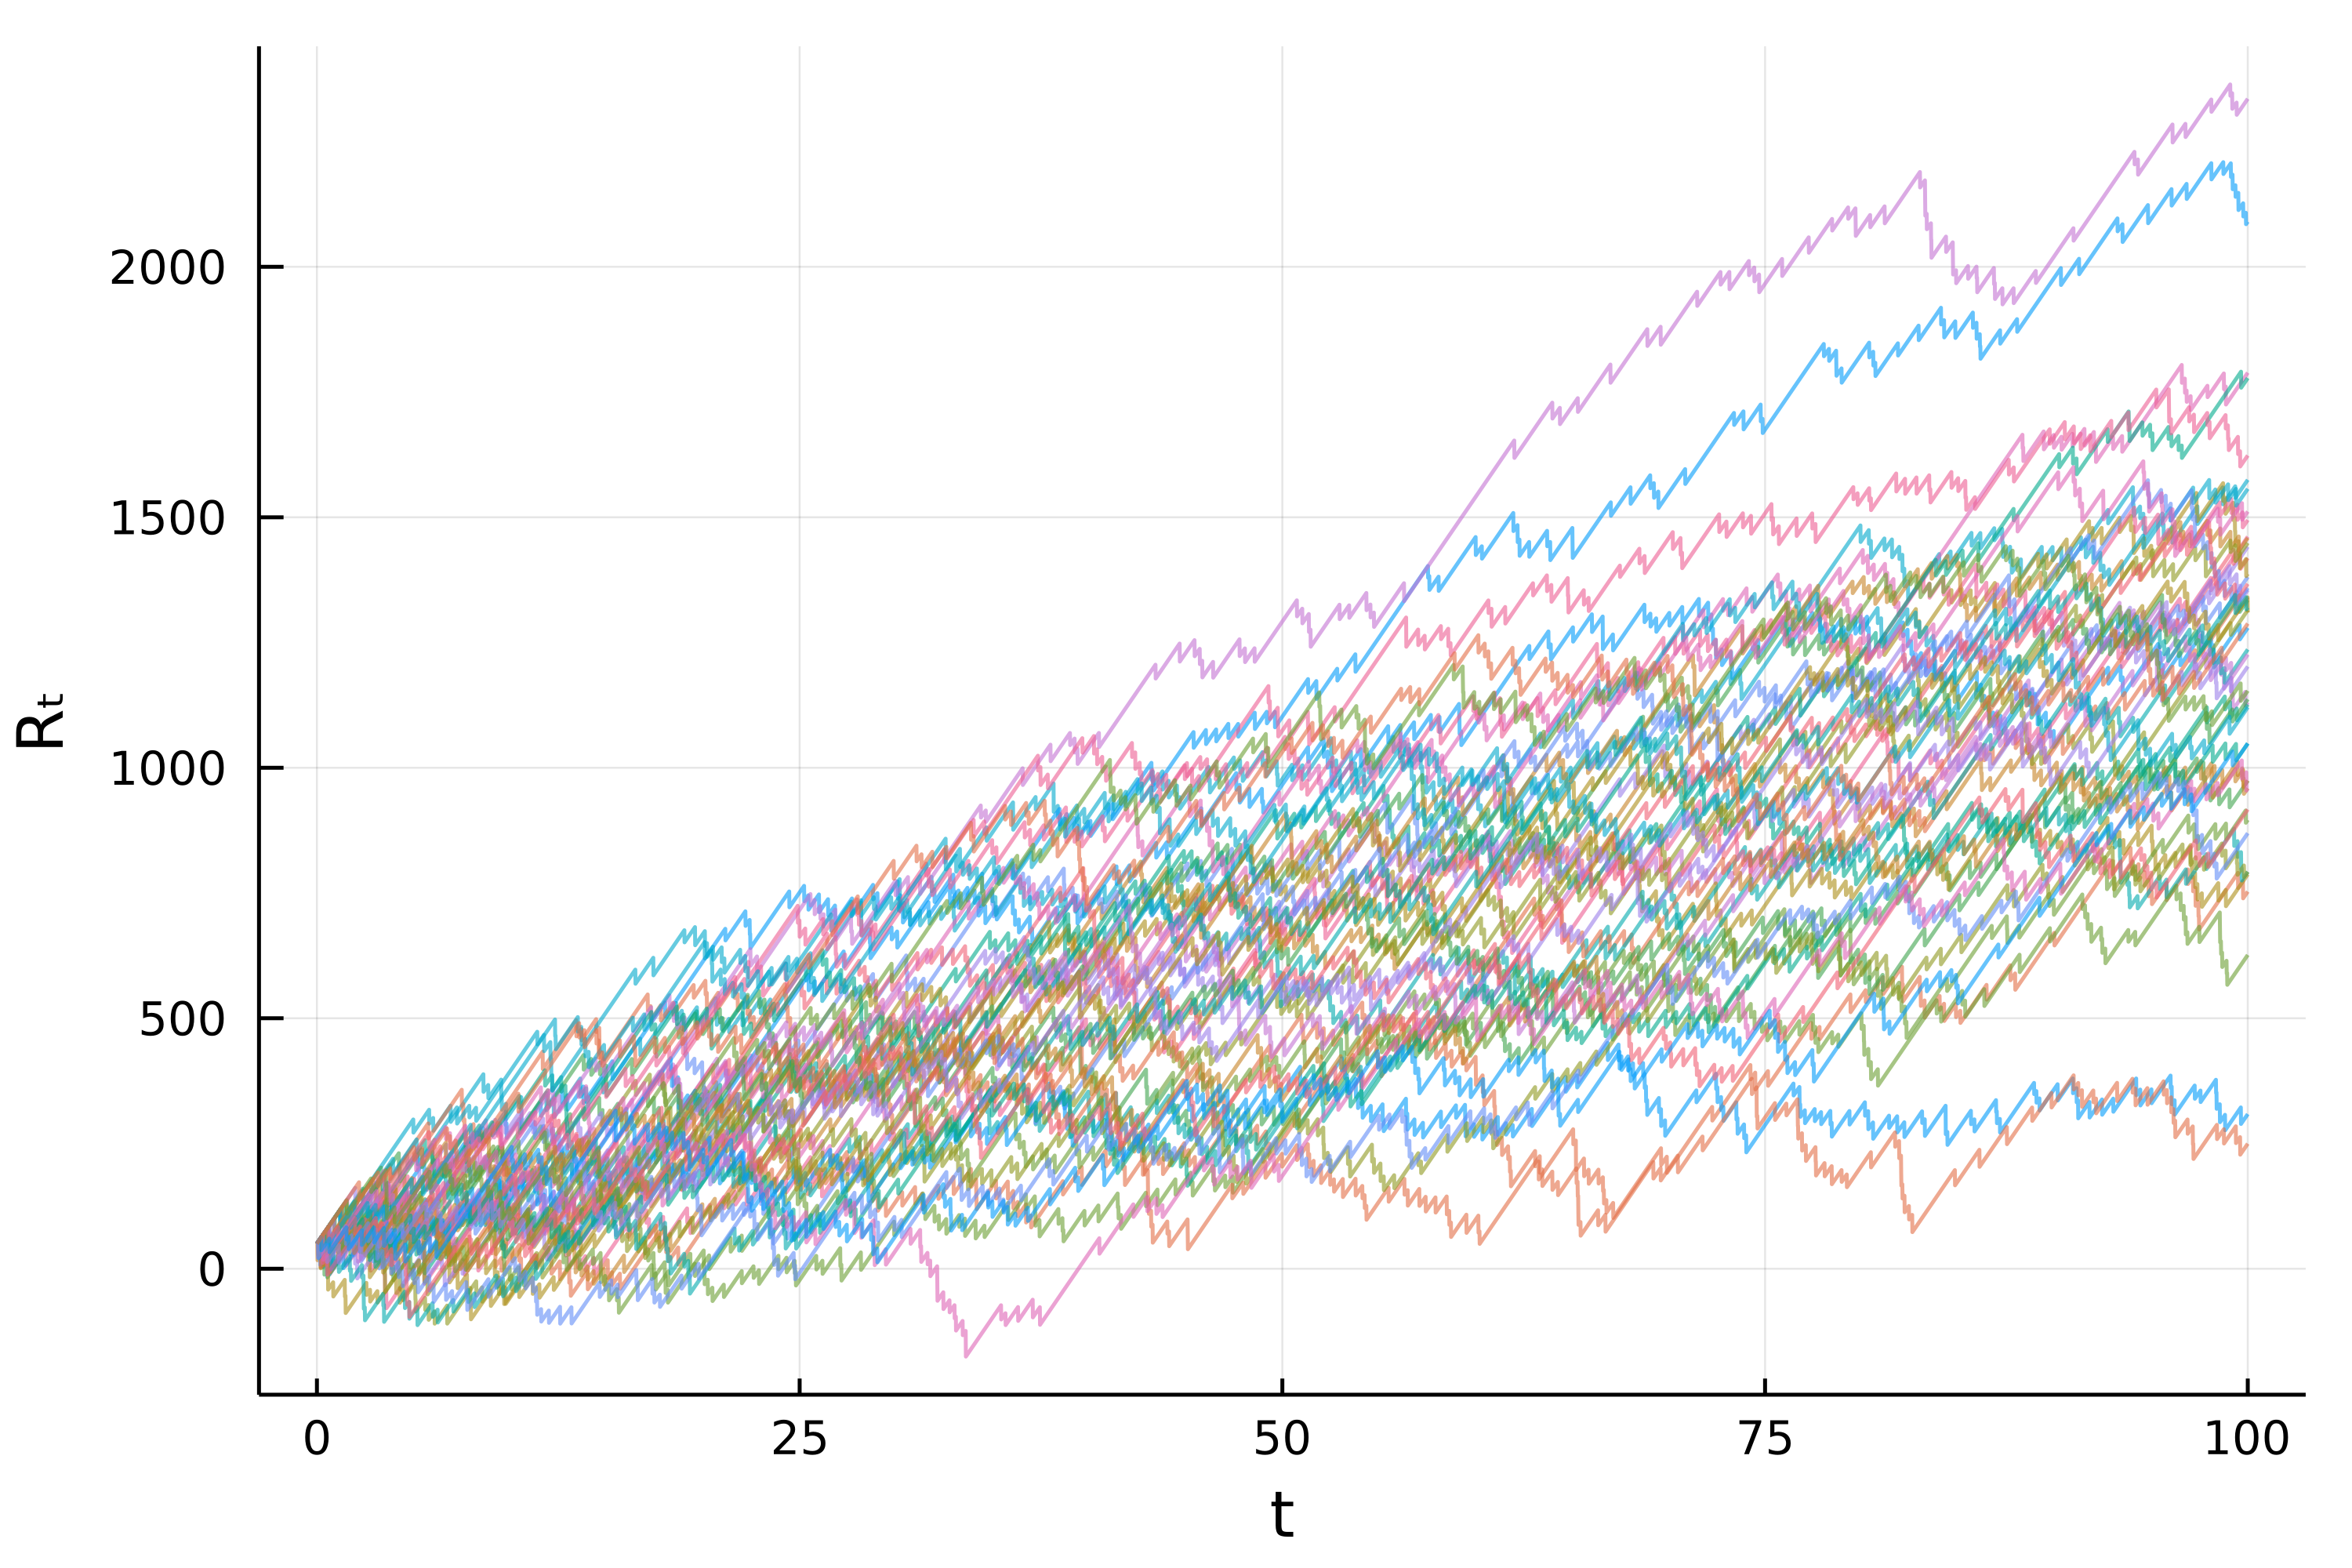
\includegraphics[scale=0.1]{fig/trajektorie.png}
		\caption{Trajektorie 50 realizacji klasycznego procesu Ryzyka zawartych w danych.}
	\end{figure}
	
	\subsubsection{Parametr {\boldmath $c$}}
	\noindent Możemy wyznaczyć go w bardzo prosty sposób. Wiedząc, że jest to współczynnik nachylenia funkcji liniowej $ct$, wystarczy, że policzymy o ile funkcja ta wzrasta w jednym kroku czasowym (obliczymy różnicę dwóch sąsiadujących danych) i wartość tę podzielimy przez długość kroku. Ważne, by upewnić się, czy w danym kroku nie nastąpił spadek. Dla pewności możemy policzyć $c$ dla kilku kroków i sprawdzić, czy otrzymane wartości są identyczne. Wartość, którą otrzymaliśmy z naszych danych to $c = 56,25$.
	
	\subsubsection{Parametr {\boldmath $\lambda$}}
	\noindent W przypadku tego parametru nie jesteśmy w stanie wyznaczyć jego dokładnej wartości, zatem skorzystamy z estymatora. Wykorzystamy fakt, że jeśli proces Poissona ma intensywność $\lambda$, to odstępy czasowe między kolejnymi skokami mają rozkład $\mathcal{E}xp(\lambda)$. Wydzielamy więc wszystkie czasy oczekiwania ze wszystkich trajektorii do jednego zbioru danych. Robimy to sumując wszystkie kroki czasowe następujące po każdym spadku aż do następnego spadku, przy czym dodajemy także ostatni krok spadkowy. Należy zaznaczyć w tym miejscu, że pozwalamy sobie tutaj na pewne uproszczenie, ponieważ przyjmujemy, że spadek miał miejsce dokładnie pod koniec kroku spadkowego, podczas gdy w rzeczywistości miał on miejsce w jego trakcie.\vspace{1.5mm}\\
	By wyestymować parametr $\lambda$, skorzystamy z faktu, że dla $\tau \sim \mathcal{E}xp(\lambda)$ wartość oczekiwana jest równa
	$$ \mathrm{E}\tau = \frac{1}{\lambda}. $$
	Najlepszym estymatorem wartości oczekiwanej jest średnia z próby. Oznaczmy przez $\tau_1, \dots, \tau_n$ odstępy czasowe pozyskane z naszych danych. Estymatorem $\lambda$ będzie więc
	$$ \widehat{\lambda} = \frac{1}{\sum\limits_{i=1}^n \tau_i}. $$
	Po obliczeniu otrzymaliśmy $\widehat{\lambda} \approx 1,48$. Poniżej możemy zobaczyć, że krzywa gęstości teoretycznej rozkładu $\mathcal{E}xp\left(\widehat{\lambda}\right)$ wyraźnie pokrywa się z histogramem z naszych danych.
	
	\begin{figure}[H]
		\centering
		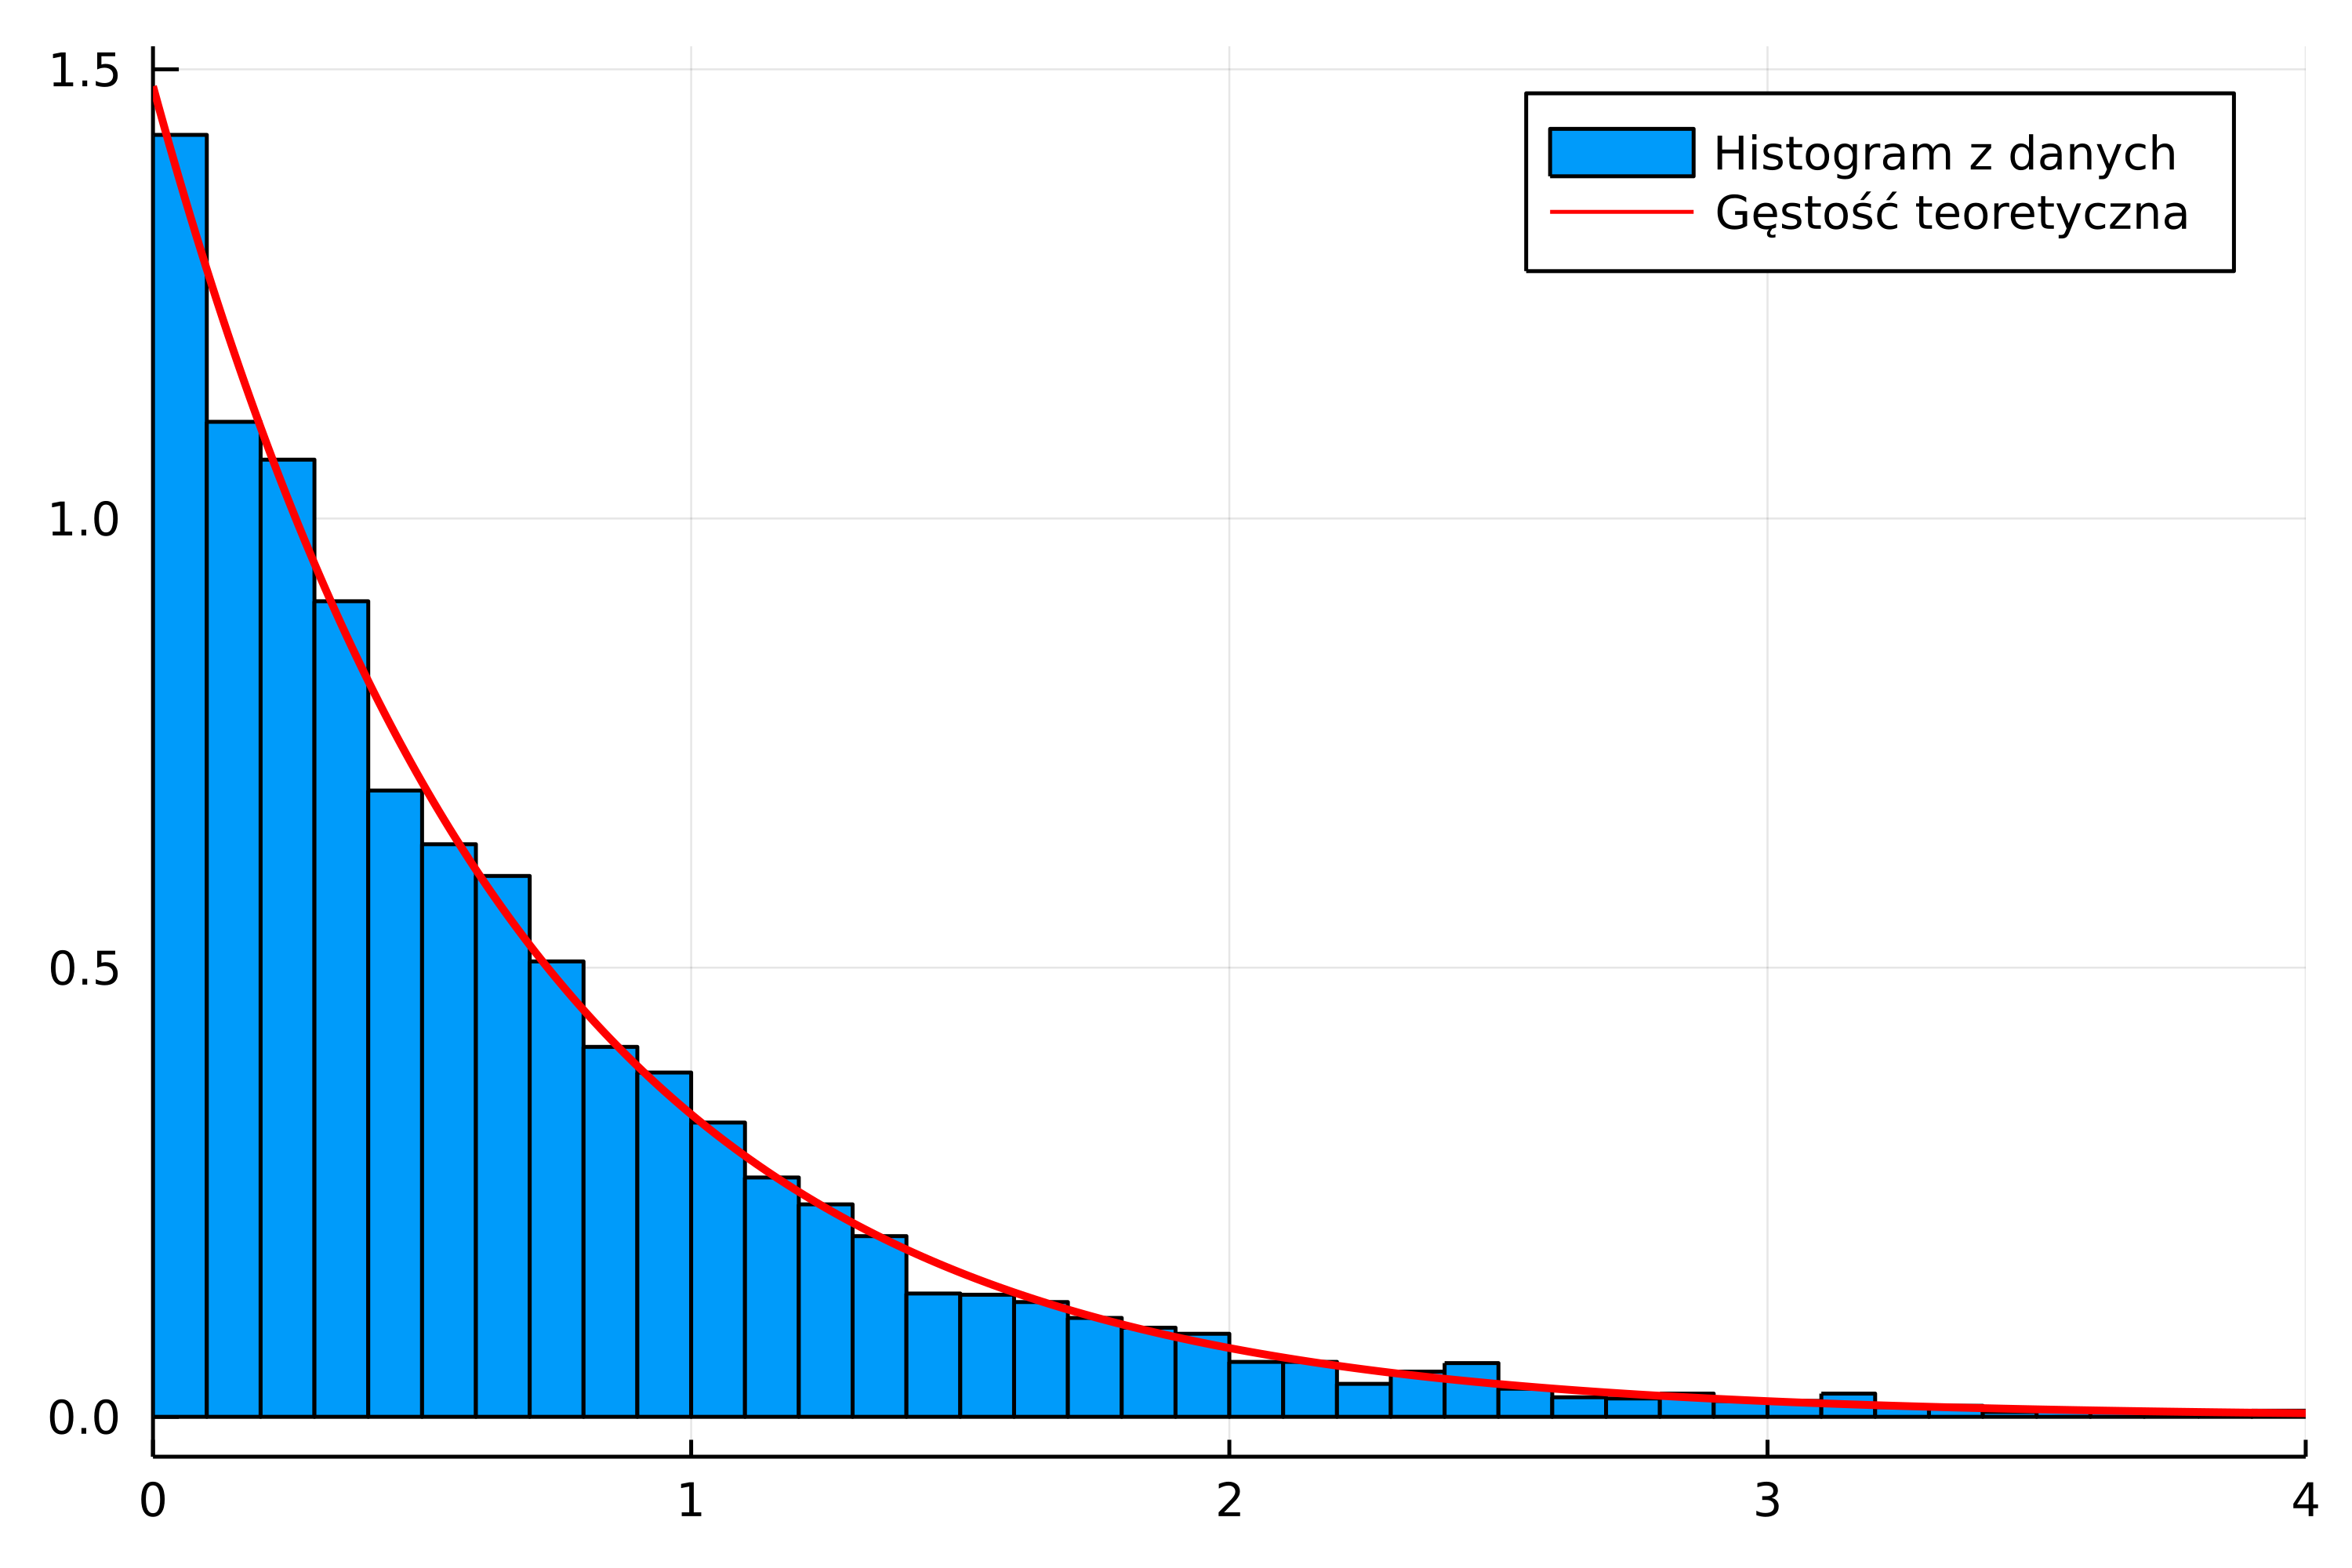
\includegraphics[scale=0.1]{fig/lambda.png}
		\caption{Porównanie unormowanego histogramu z odstępów czasowych pomiędzy skokami z gęstością teoretyczną rozkładu $\mathcal{E}xp\left(\widehat{\lambda}\right)$.}
	\end{figure}
	
	\subsubsection{Straty {\boldmath $X_i$}}
	\noindent Niezbędną informacją potrzebną do dopasowania modelu do badanego procesu Ryzyka jest rozkład strat $X_i$. Aby pozyskać dane opisujące straty, obliczmy różnicę sąsiadujących danych w każdym kroku spadkowym. Dodatkowo, ponieważ nasze dane opisują trajektorie z dokładnością do kroku czasowego, to należy do otrzymanych wartości dodać jeszcze przyrost z przychodów w tym kroku. W naszym przypadku przyrost ten będzie wynosił $c \cdot h = 0,56625$.
	
	\begin{figure}[H]
		\centering
		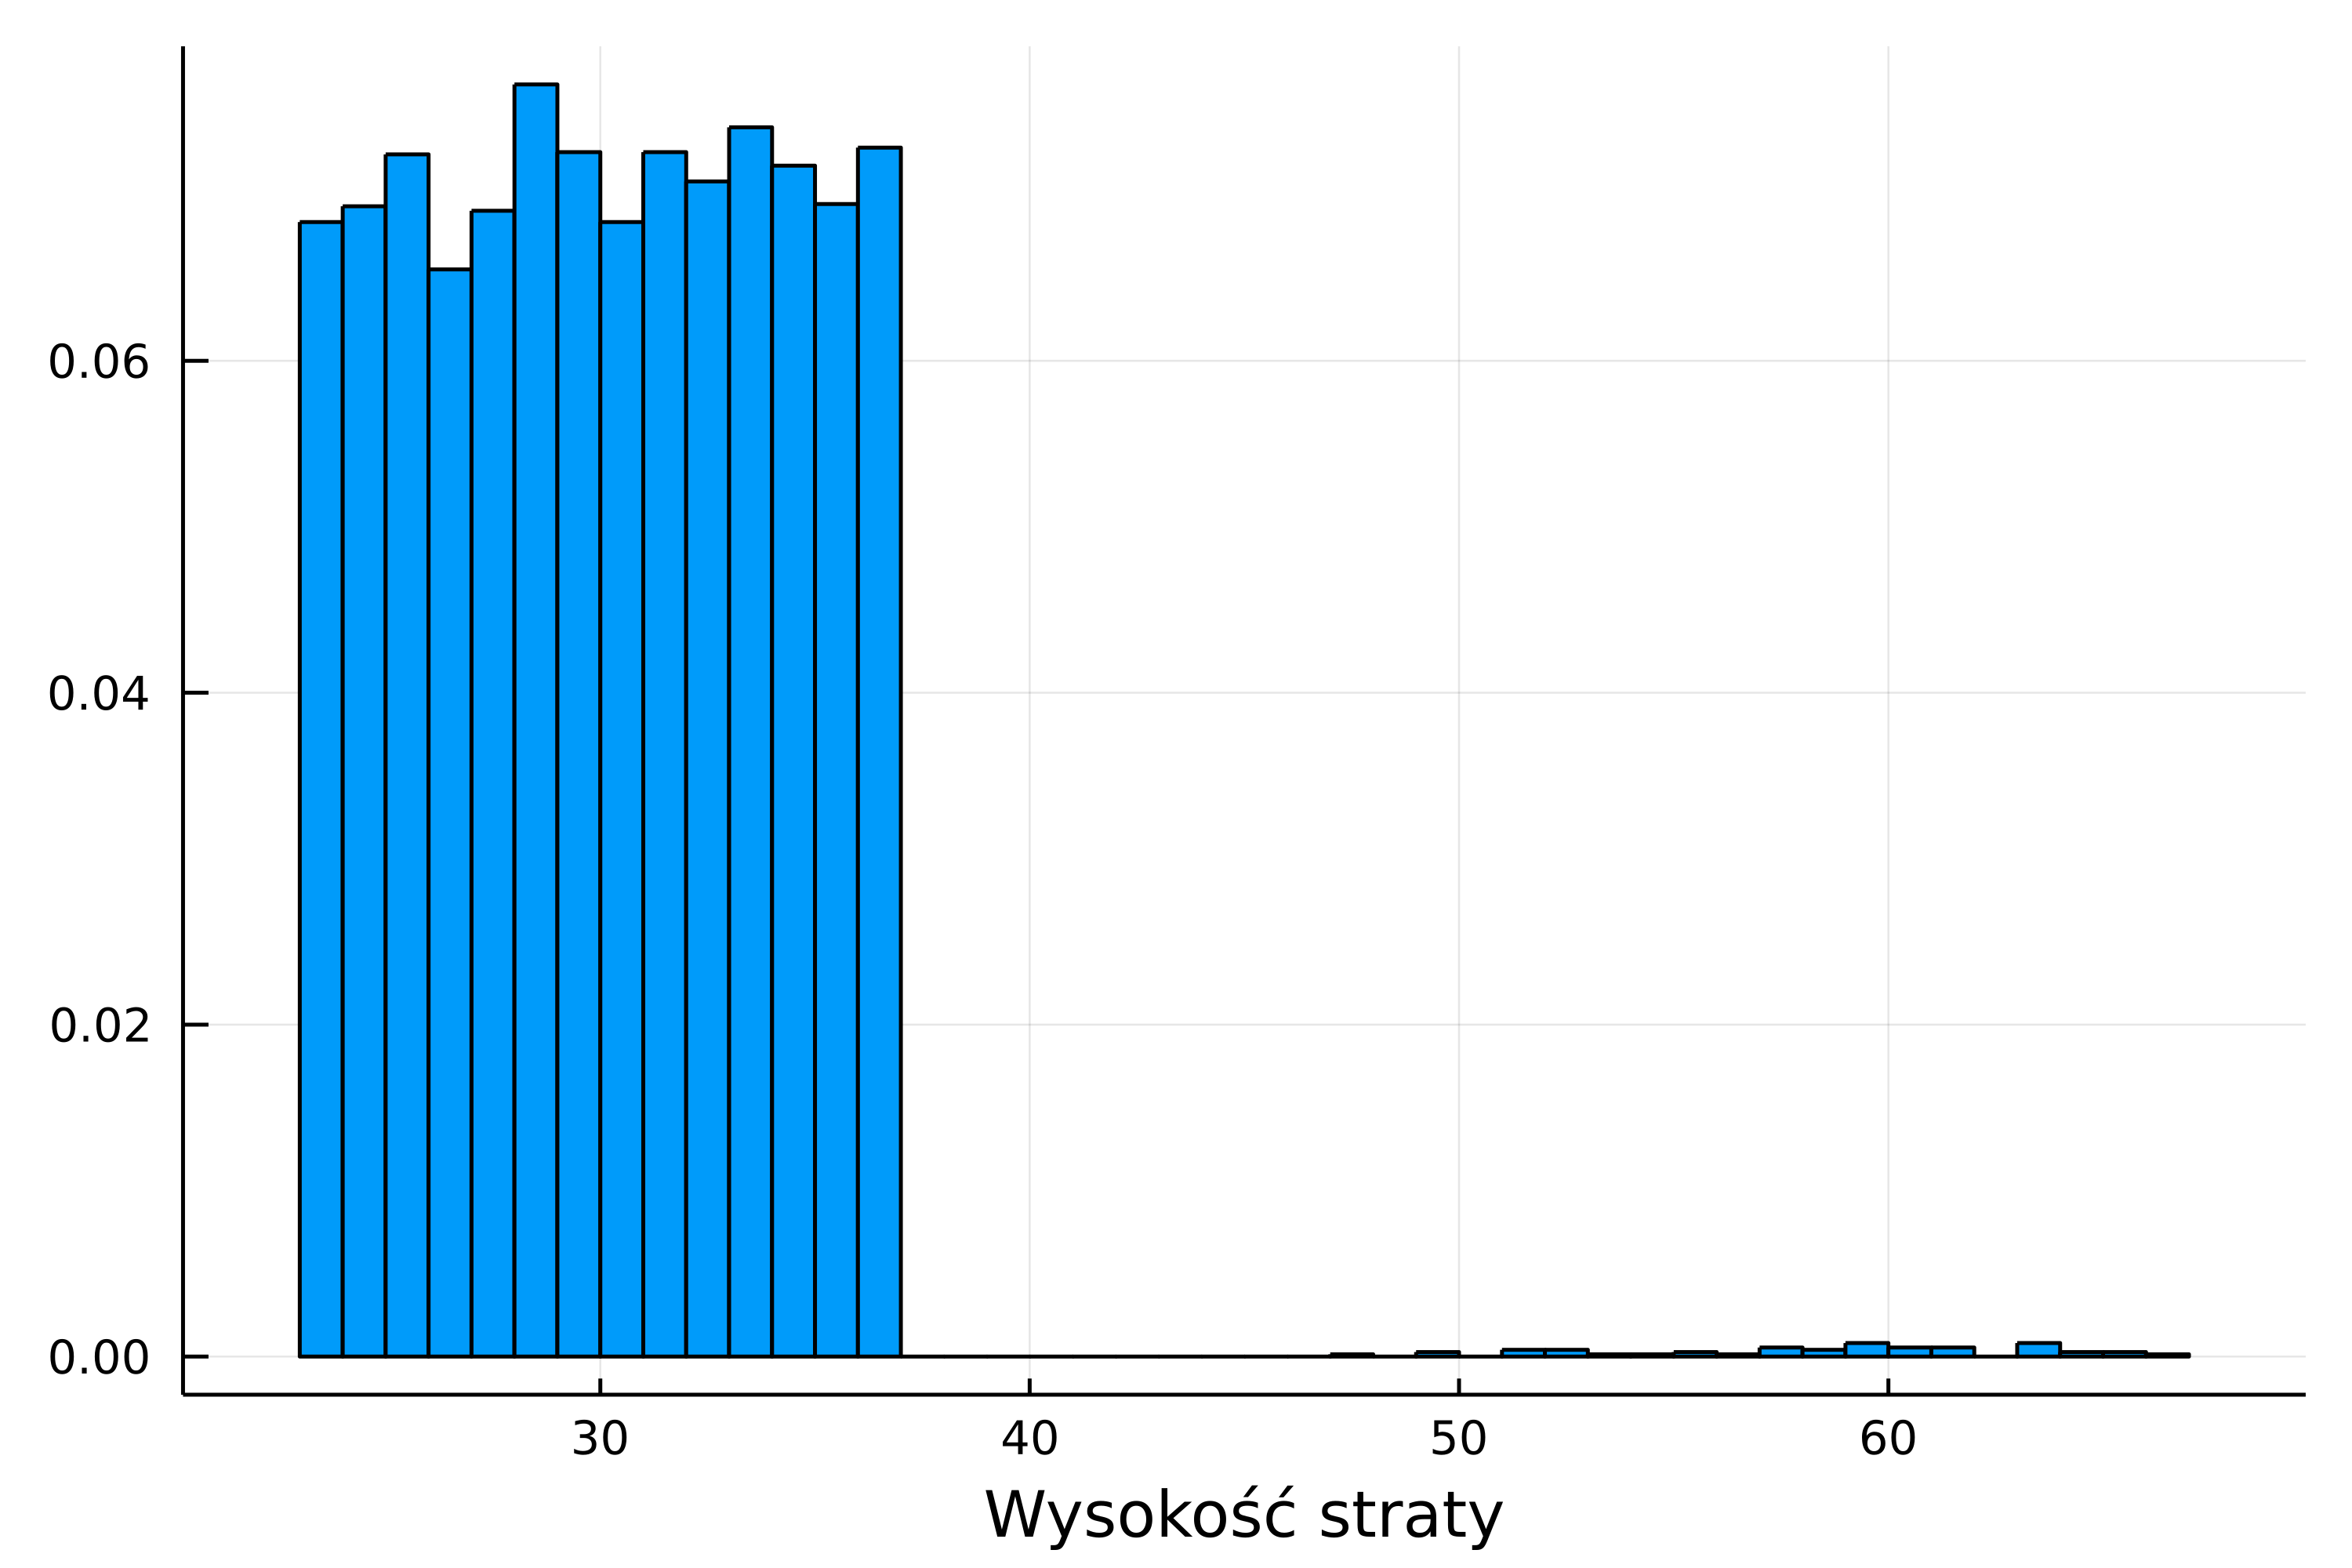
\includegraphics[scale=0.1]{fig/straty_1.png}
		\caption{Unormowany histogram ze wszystkich strat pozyskanych z 50 trajektorii.}
	\end{figure}

	\noindent Na powyższym histogramie widzimy, że zdecydowana większość danych znajduje się w okolicach 30. Kształt histogramu sugeruje, że mają one rozkład jednostajny. Możemy jednak zauważyć, że pojawia się niewielka ilość odstających większych wartości.
	
	\begin{figure}[H]
		\centering
		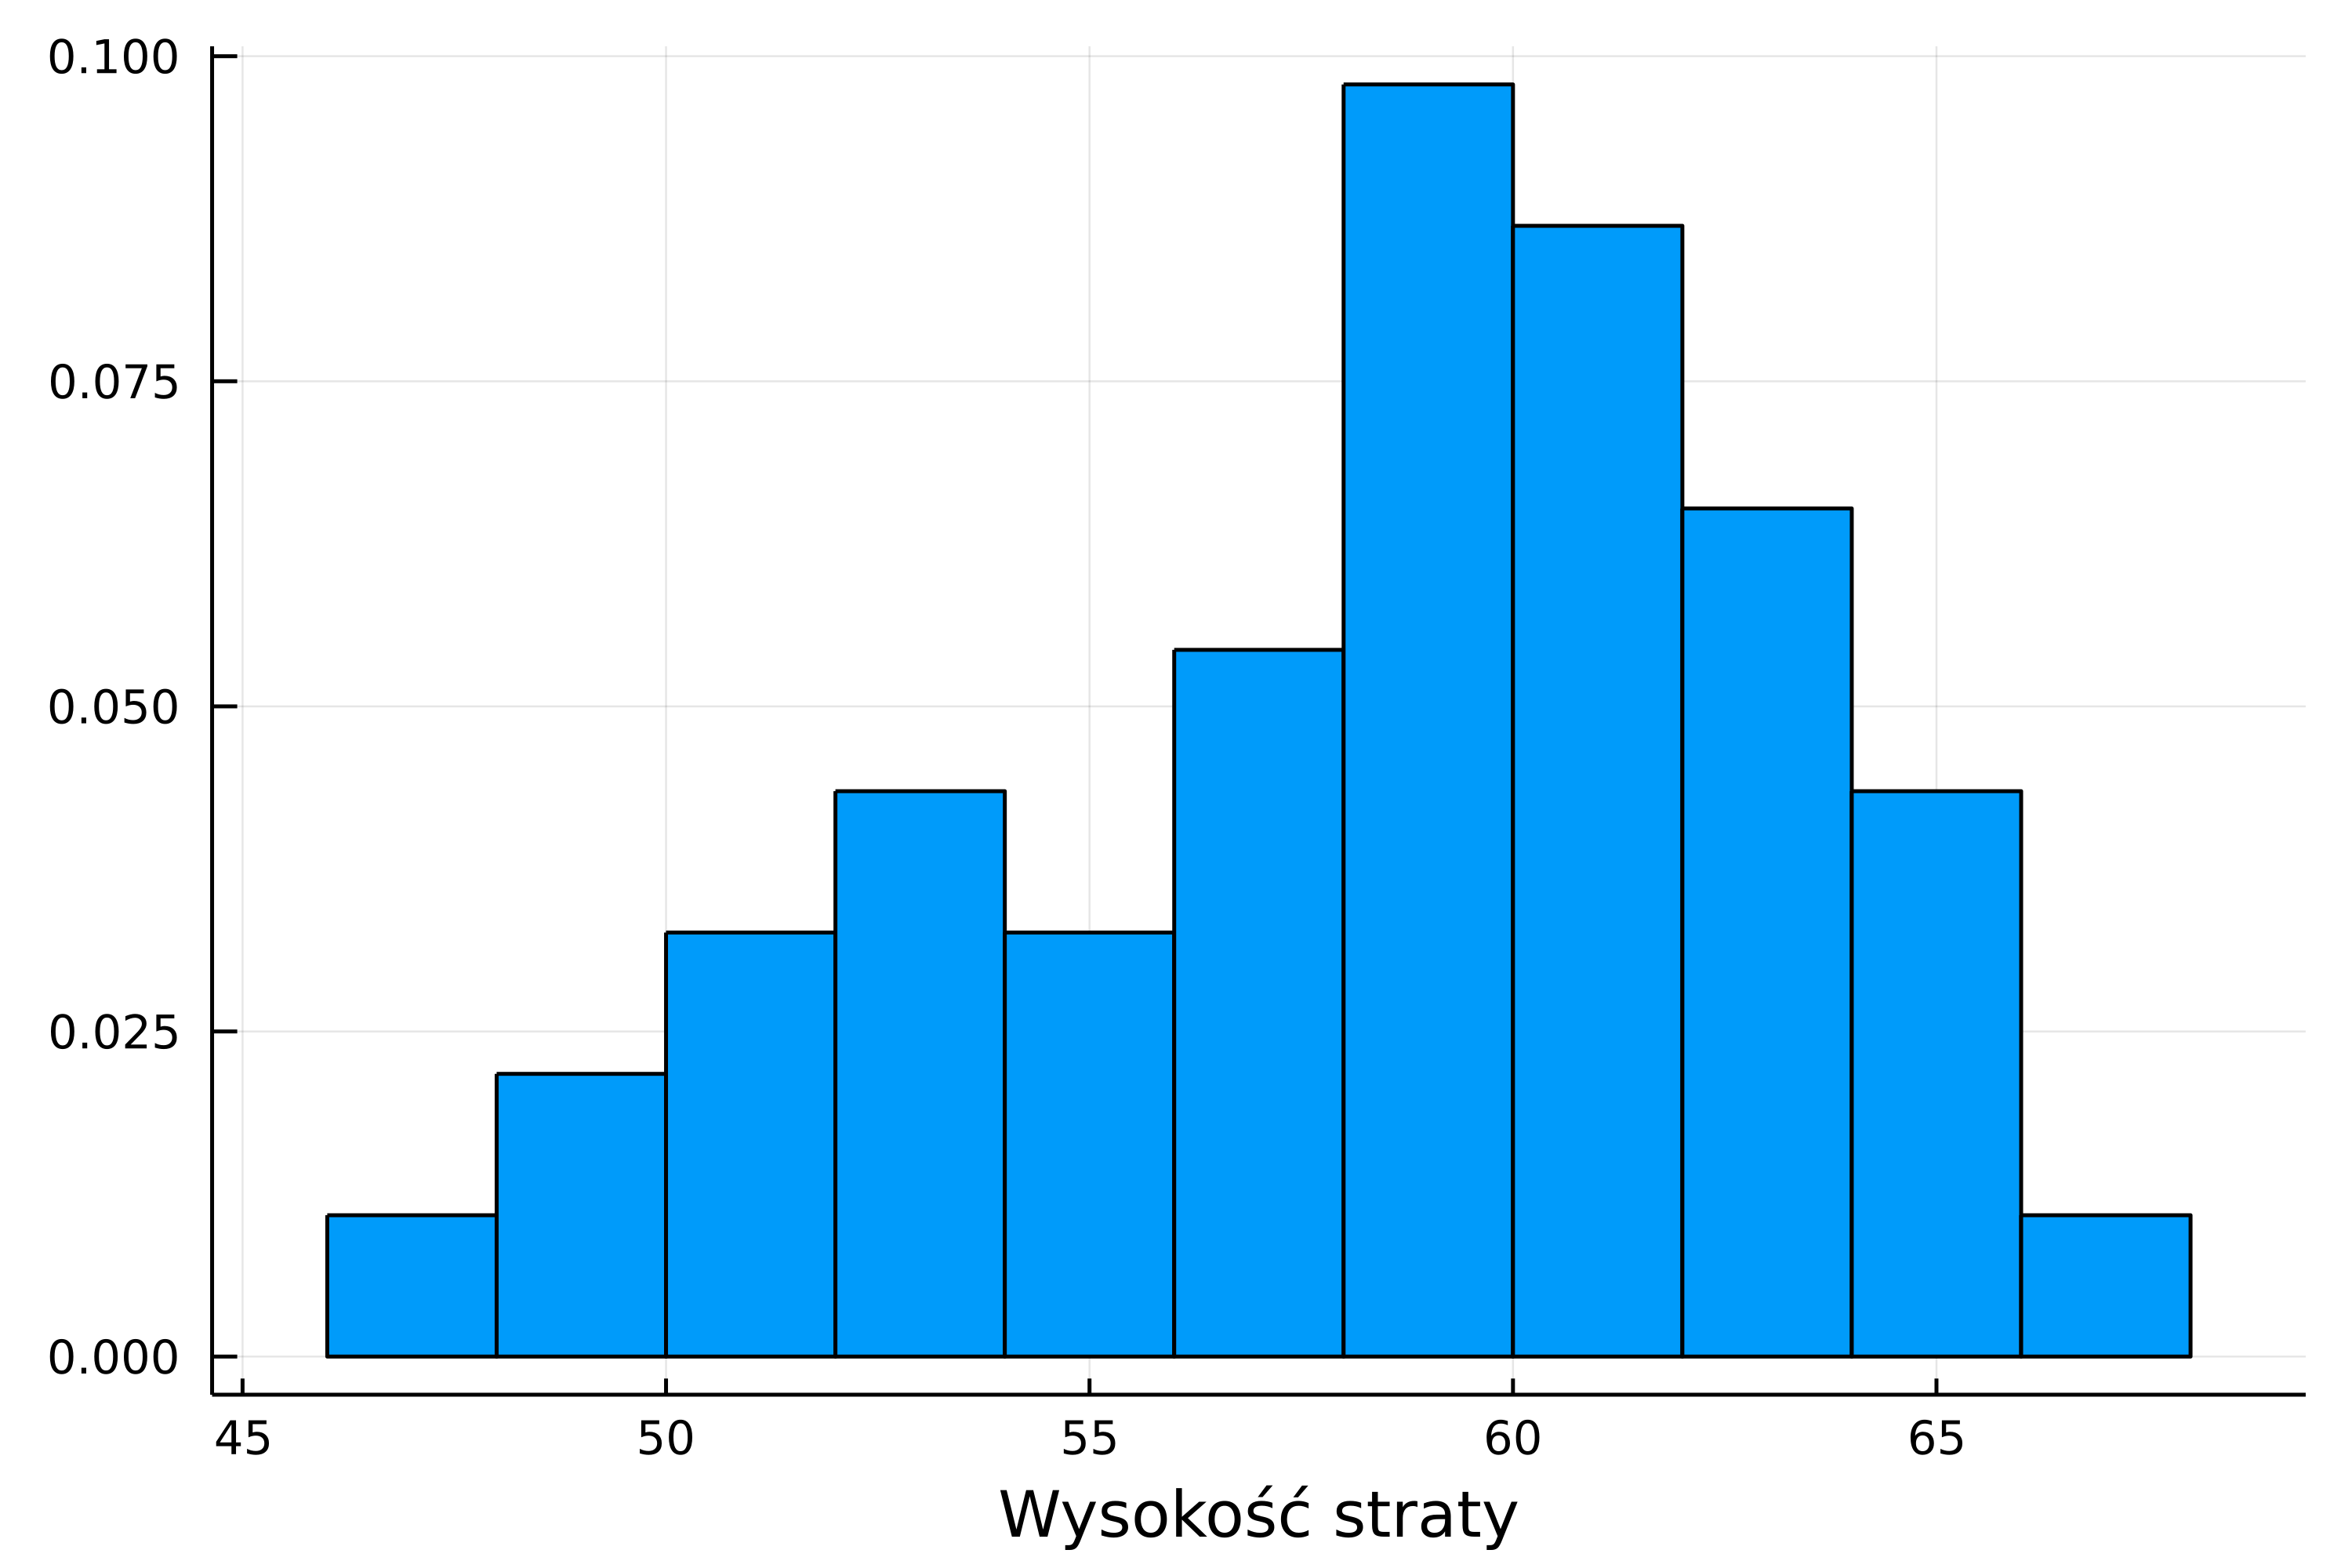
\includegraphics[scale=0.1]{fig/straty_2.png}
		\caption{Unormowany histogram ze strat większych od 40}
	\end{figure}

	\noindent Wspomnianych wartości odstających jest zaledwie 46 na 7358 wszystkich danych. 


	
	\subsubsection{Parametr {\boldmath $\theta$}}
	
	
	
	\subsection{Prawdopodobieństwo ruiny}
	
	
	
	
	\section{Zadanie 2}
	\subsection{Proces Wienera}
	\noindent Procesem Wienera (Ruchem Browna) nazywamy proces $\{W_t\}_{t\geqslant0}$, który spełnia:
	\begin{itemize}[leftmargin=10mm]%, label=$\boldsymbol{\cdot}$]
		\item $W_0=0$,
		\item $W_t$ ma niezależne przyrosty,
		\item $W_t$ ma stacjonarne przyrosty,
		\item $W_t \sim \mathcal{N}(0, t)$,
		\item $W_t$ ma ciągłe trajektorie.
	\end{itemize}	
	\noindent \textbf{Algorytm}\\
	\noindent Naszym celem jest wygenerowanie wektora $\left[W_{t_0}, W_{t_1}, \dots, W_{t_n}\right]$, gdzie
	\begin{equation}
		t_i=ih, \quad i=0,1,\dots,n, \quad h=T/n
	\end{equation}
	\begin{equation}
		t_i=ih, \quad i\in\left[n\right]=\left\{0, 1, \dots, n\right\}, \quad h=T/n
	\end{equation}
	\begin{equation}
		t_i=ih, \quad i\in\mathbb{N}_0^{\leqslant n}, \quad h=T/n.
	\end{equation}
	W tym celu stosujemy poniższy algorytm
	\begin{enumerate}[leftmargin=10mm]
		\item Generuj realizację zmiennych $\xi_i\text{ iid }\mathcal{N}(0,1), \,i\in\left[n-1\right]$,
		\item $W_{t_0}=W\left(0\right)=0$,
		\item $W_{t_{i+1}} = W_{t_{i}}+\sqrt{h}\xi_i,\quad i\in\left[n-1\right]$%\in\mathbb{N}^{n}$.
	\end{enumerate}

	\subsection{Średni czas wyjścia procesu Wienera}
	\noindent Niech $\left\{B^x_t\right\}_{t\geqslant0}$ będzie ruchem Browna startującym z $x\in\mathbb{R}$, a $\tau^x$ czasem wyjścia tego procesu z ustalonego przedziału $[a, b]$, czyli
	\begin{equation}
		\tau^x=\inf\left\{t\geqslant0:B^x_t\notin[a, b]\right\}
	\end{equation}
	\noindent dla $x$ z przedziału $[a,b]$. Łatwo można pokazać, że $B^{x+y}_t\in[a ,b] \iff B^x_t\in[a-y, b-y]$.
%	\\Ponieważ $W_t+x\in[a, b] \iff W_t\in[a-x, b-x]$ \\
%	$B^x_t\in[a,b]\iff B^y_t\in[a-x+y, b-x+y]$\\widzimy, że czas wyjścia nie zależy bezpośrednio od wyboru punktów $a$ oraz $b$, a od punktu początkowego oraz długości przedziału.
	Dodatkowo, ponieważ ruch Browna jest $\frac{1}{2}$-samopodobny($W_t\overset{d}{=}\sqrt{\Delta}W_{t/\Delta}$), zachodzi
	\begin{equation}
		B^x_t=W_t+x\overset{d}{=}\Delta W_{t/\Delta^2}+x = \Delta\left(W_{t/\Delta-\frac{x}{\Delta}}\right)=B^{x/\Delta}_{t/\Delta^2}
	\end{equation}
	Korzystając z tych dwóch własności pokażemy, że
	\begin{equation}
		\begin{split}
			\tau^x&\overset{d}{=}\inf\left\{\Delta^2\frac{t}{\Delta^2}\geqslant0:\Delta B^{x/\Delta}_{t/\Delta^2}\notin[a, b]\right\} =\Delta^2\inf\left\{t^*\geqslant0:B^{x/\Delta}_{t^*}\notin\left[\frac{a}{\Delta},\frac{b}{\Delta}\right]\right\}\\
			&=\Delta^2\inf\left\{t^*\geqslant0:B^{(x-y)\Delta}_{t^*}\notin\left[\frac{a-y}{\Delta},\frac{b-y}{\Delta}\right]\right\}
		\end{split}
	\end{equation}
	Wybierając teraz $\Delta=(b-a)$ oraz $y=a$ otrzymujemy
	\begin{equation}\label{eq:tau_przeskalowane}
		\tau^x\overset{d}{=}(b-a)^2\inf\left\{t\geqslant0:B^z_t\in[0,1]\right\},
	\end{equation}
	gdzie $z$ jest "przeskalowanym" $x$ na odcinek $[0, 1]$.\\
	Dzięki tym przekształceniom widzimy, że $\mathbb{E}\tau^x$ zwiększa się z kwadratem długości przedziału jaki rozważamy oraz zależy ona od odległości $x$ od jednego końca przedziału względem drugiego. Z tego powodu później będziemy rozważać jedynie czas wyjścia z przedziału $[0, 1]$.
	
	
	
	
%	Naszym celem jest oszacowanie średniego czasu wyjścia procesu Wienera startującego z $x\in\mathbb{R}$, w zależności od wyboru $x$.

















	\newpage
	
	\section{Podsumowanie}
	
	
	
	\newpage
	\begin{thebibliography}{1}
		\bibitem{dane}
		\url{}
	\end{thebibliography}


\end{document}